
\documentclass[preprint,10pt]{elsarticle}

\usepackage{epsfig}
\usepackage{amsmath,amssymb,bm}
\usepackage{hyperref}


\journal{...}

\begin{document}

\begin{frontmatter}
\title{Probing photonic content of the proton using photon-induced dilepton production in $p+Pb$ collisions at the LHC}


\author{M. Dyndal}
\address{DESY}
\author{A. Glazov}
\address{DESY}
\author{M. Luszczak}
\address{...}
\author{R. Sadykov}
\address{...}



\begin{abstract}
We propose a new experimental method of validating photon PDF of the proton at LHC energies.
\end{abstract}


%%\keywords{QED, Equivalent Photon Approximation, LHC}

\end{frontmatter}


%%%%%%%%%%%%%%%%%%%%%%%%%%%%%%%%%%
%%%%%%%%%%%%%%%%%%%%%%%%%%%%%%%%%%
\section{Introduction}
%%%%%%%%%%%%%%%%%%%%%%%%%%%%%%%%%%

A significant fraction of proton-proton collisions at the LHC involves quasi-real photon interactions.

...~\cite{Chatrchyan:2011ci}


As the signal process does not involve the exchange of color with the photon-emitting nucleus, no significant particle production is expected in the rapidity region between the dilepton system and the nucleus. 
The photon-emitting nucleus is also expected to produce no neutrons because the photons couple to the entire nucleus. 
Thus a combination of a rapidity gap and zero neutrons in the same direction provide straightforward criteria to identify these events experimentally. 

%%%%%%%%%%%%%%%%%%%%%%%%%%%%%%%%%%
\section{Formalism}
%%%%%%%%%%%%%%%%%%%%%%%%%%%%%%%%%%

%-------------------------------------
\subsection{Elastic photon fluxes}
%-------------------------------------


To get the distribution of the elastic photons from the proton, one can express the equivalent photon flux through
the electric and magnetic form factors $G_E(Q^2)$ and $G_M(Q^2)$ of the proton.
This contribution is obtained as
\begin{eqnarray}
   \gamma^{p}_{el}(x,Q^2) = \frac{\alpha_{\rm{em}}}{\pi}
\Big[ \Big( 1- {x \over 2} \Big)^2 \, {4 m_p^2 G_E^2(Q^2) + Q^2 G_M^2(Q^2) \over 4m_p^2 + Q^2} + {x^2 \over 4} G_M^2(Q^2) \Big]~,
\label{proton_el_flux}
\end{eqnarray}
where $x$ is the momentum fraction of the proton taken by the photon, $Q^2$ is the photon virtuality, $\alpha_{\rm{em}}$ is the electromagnetic structure constant and $m_p$ is the proton mass.

To express the elastic photon flux for the nucleus ($\gamma^{\rm Pb}_{el}$), we follow Ref.~\cite{Budnev:1974de} and replace 
\begin{eqnarray}
 {4 m_p^2 G_E^2(Q^2) + Q^2 G_M^2(Q^2) \over 4m_p^2 + Q^2} \longrightarrow Z^2 F_{\rm em}^2(Q^2)~,
 \end{eqnarray}
where $F_{\rm em}(Q^2)$ is the electromagnetic form factor of the nucleus and $Z$ is its charge.
We also neglect the magnetic form factor of the ion in the following.

For the Pb nucleus, we use the form factor parameterization from the STARlight MC generator~\cite{Klein:2016yzr}:
%%
\begin{eqnarray}
 F_{\rm em}(Q^2) = {3 \over (QR_A)^3}\Big[ \sin(QR_A) - QR_A \cos(QR_A) \Big] { 1 \over 1 + a^2 Q^2}~,
\end{eqnarray}
%%%
where $R_A = 1.1 A^{1/3}$ fm, $a = 0.7$ fm and $Q = \sqrt{Q^2}$.
%%%

The elastic photon PDFs of the proton and lead nucleus can be integrated over $Q^2$ as 
\begin{equation}
\gamma^{(p,Pb)}_{el}(x)  = \int d Q^2 \gamma^{(p,Pb)}_{el}(x, Q^2) \,.
\end{equation}
This is useful for the collinear-factorization approach since the $Q^2$ dependence factorizes in this case. 
%-----------------------------------------------------------
\subsection{Collinear-factorization approach and choice of the scale}
%-----------------------------------------------------------

The inelastic processes, with breakup of a proton, can be also considered.
At LO and at a given scale $\mu^2$, the photon parton distribution $\gamma^p_{inel}(x,\mu^2)$ of photons carrying a fraction $x$ of the proton's momentum, obeys the DGLAP equation:
%%
\begin{eqnarray}
{d \gamma^p_{inel}(x,\mu^2) \over d \log \mu^2} =&& {\alpha_{\rm{em}} \over 2 \pi} \int_x^1 {dy \over y} 
\Big [ \sum_q P_{\gamma \leftarrow q}(y) 
 q ({x \over y}, \mu^2 )   + P_{\gamma \leftarrow \gamma}(y) \gamma^p_{inel}({x \over y},\mu^2) \Big ]~,
\end{eqnarray}
%%
where $q (x,\mu^2)$ is the quark PDF,  $P_{\gamma \leftarrow q}$ is the $q\rightarrow\gamma$ splitting function, and $P_{\gamma \leftarrow \gamma}$ corresponds to the virtual self-energy correction to the photon propagator.
This is the basis for colinear photon-PDFs in the initial~\cite{Gluck:2002fi, Martin:2004dh} and more recent~\cite{Ball:2013hta, Martin:2014nqa, Schmidt:2014aba, Harland-Lang:2016kog, Giuli:2017oii, Manohar:2016nzj, Bertone:2017bme} analyses.

The computation of the photon-induced dilepton production cross section  requires definition of the  scale ($\mu^2$) at which the photon PDFs are convoluted.
The usual choice for $\mu$ is the mass of the system (motivated by the $s$-channel quark--antiquark annihilation process) or the transverse momentum of the leading object. 
These choices are however not optimal for the $t$- and $u$-channel initiated photon-induced process.
By analogy to DIS (Fig.~\ref{fig:diagrams}), where the scale is associated with the virtuality of the exchanged photon,
it is possible to define the scale in case of the $\gamma\gamma\rightarrow\ell^+\ell^-$ process.
This is achieved by taking the virtuality of the massive $t$- or $u$-channel propagator (Fig.~\ref{fig:diagrams}b or c).
Hence, $\mu^2 = -(p^{\gamma^{Pb}}-p^{\ell^-})^2$ for the $t$-channel diagram and $\mu^2 = -(p^{\gamma^{Pb}}-p^{\ell^+})^2$ for the $u$-channel exchange, where $p^{\gamma^{Pb}}$ is the four momentum
of the photon emitted by lead and $p^{\ell^{\pm}}$ is the four momentum of the lepton of the corresponding charge.
Note that the $u$- and $t$- channel diagrams have vanishing interference in the zero lepton mass limit. Therefore, they can be separated  while convoluting PDFs with the partonic cross section.

In the collinear approach, the $p+\textrm{Pb}\rightarrow \textrm{Pb} + \ell^+\ell^- + X$ production cross section can be written as
%
\begin{equation}
\sigma 
= S^2 \int dx_p dx_{\rm Pb} 
\Big [ \gamma^{p}_{el}(x_p) + \gamma^{p}_{inel}(x_p,\mu^2) \Big]
 \gamma^{\rm Pb}_{el}(x_{\rm Pb})
\sigma_{\gamma \gamma \rightarrow \ell^+ \ell^-}(x_p, x_{\rm Pb}) \,,
\label{collinear_factorization_formula}
\end{equation}
%
where $\sigma_{\gamma \gamma \rightarrow \ell^+ \ell^-}$
is the elementary cross section for the $\gamma \gamma \rightarrow \ell^+ \ell^-$ subprocess and $S^2$ is the so-called survival factor which takes into account the requirement that there be no hadronic interactions between the proton and the ion.


%%%%%%%%%%%%%%%%%%%%%%%%%%%%%%%%%%
\section{Fiducial selection and possible background}
%%%%%%%%%%%%%%%%%%%%%%%%%%%%%%%%%%



%%%%%%%%%%%%%%%%%%%%%%%%%%%%%%%%%%
\section{Results with collinear photon-PDFs}
%%%%%%%%%%%%%%%%%%%%%%%%%%%%%%%%%%

We start with the calculation of the elastic contribution, $p+\textrm{Pb}\rightarrow p+\textrm{Pb}+ \ell^+\ell^-$.
In this case the photon flux becomes:
\begin{equation}
f_\gamma^{p}(x,\mu) = f_\gamma^{p}(x) 
\end{equation}
and the following parameterization is used~\cite{}:
\begin{equation}
f_\gamma^{p}(x) = \frac{\alpha}{\pi}
\left(
\frac{1-x+0.5x^2}{x}
\right)
\left(
\frac{A+3}{A-1}\log{A}-\frac{17}{6}-\frac{4}{3A}+\frac{1}{6A^2}
\right)~,
\end{equation}
where $A = 1+\frac{Q_0^2(1-x)}{x m_p^2}$ and $Q_0^2 = 0.71$~\GeV$^2$.

The results for the elastic case are cross-checked with the calculation from STARlight MC and a good agreement is found:
$\sigma_{fid}^{\textrm{el}} = 17.5$~nb, whereas $\sigma_{fid}^{\textrm{STARlight}} = 17.0$~nb.
Both calculations are also corrected by a factor $S^2=0.96$ which takes into account the requirement that there be no hadronic interactions between the proton and the ion. This is calculated using STARlight, where the hard-sphere proton--nucleus requirement~\cite{Klein:2016yzr} is used.

Next, for the inelastic case ($\gamma p\rightarrow \ell^+\ell^- + X$), several recent parameterizations of the photon parton distributions are studied: CT14qed~\cite{Schmidt:2015zda}, LUXqed17~\cite{Manohar:2017eqh} and NNPDF3.1luxQED~\cite{Bertone:2017bme}.
Comparison of several lepton kinematic distributions between different photon-PDFs are shown in Fig.~\ref{fig:elastic},\ref{fig:elastic_cut},\ref{fig:inc},\ref{fig:inc_cut}.

\begin{figure}[h!]
\includegraphics[width=0.4\textwidth]{figures/Mll_elastic.pdf}
\includegraphics[width=0.4\textwidth]{figures/RatioMll_elastic.pdf}
\includegraphics[width=0.4\textwidth]{figures/Yll_elastic.pdf}
\includegraphics[width=0.4\textwidth]{figures/RatioYll_elastic.pdf}
\includegraphics[width=0.4\textwidth]{figures/pTl_elastic.pdf}
\includegraphics[width=0.4\textwidth]{figures/RatiopTl_elastic.pdf}
\includegraphics[width=0.4\textwidth]{figures/etal_elastic.pdf}
\includegraphics[width=0.4\textwidth]{figures/Ratioetal_elastic.pdf}
\caption{Elastic distributions (the only cut is on leptons $p_T$)}
\label{fig:elastic}
\end{figure}

\begin{figure}[h!]
\includegraphics[width=0.4\textwidth]{figures/Mll_elastic_cut.pdf}
\includegraphics[width=0.4\textwidth]{figures/RatioMll_elastic_cut.pdf}
\includegraphics[width=0.4\textwidth]{figures/Yll_elastic_cut.pdf}
\includegraphics[width=0.4\textwidth]{figures/RatioYll_elastic_cut.pdf}
\includegraphics[width=0.4\textwidth]{figures/pTl_elastic_cut.pdf}
\includegraphics[width=0.4\textwidth]{figures/RatiopTl_elastic_cut.pdf}
\includegraphics[width=0.4\textwidth]{figures/etal_elastic_cut.pdf}
\includegraphics[width=0.4\textwidth]{figures/Ratioetal_elastic_cut.pdf}
\caption{Elastic distributions (fiducial region)}
\label{fig:elastic_cut}
\end{figure}

\begin{figure}[h!]
\includegraphics[width=0.4\textwidth]{figures/Mll_inc.pdf}
\includegraphics[width=0.4\textwidth]{figures/RatioMll_inc.pdf}
\includegraphics[width=0.4\textwidth]{figures/Yll_inc.pdf}
\includegraphics[width=0.4\textwidth]{figures/RatioYll_inc.pdf}
\includegraphics[width=0.4\textwidth]{figures/pTl_inc.pdf}
\includegraphics[width=0.4\textwidth]{figures/RatiopTl_inc.pdf}
\includegraphics[width=0.4\textwidth]{figures/etal_inc.pdf}
\includegraphics[width=0.4\textwidth]{figures/Ratioetal_inc.pdf}
\caption{Inclusive distributions (the only cut is on leptons $p_T$)}
\label{fig:inc}
\end{figure}

\begin{figure}[h!]
\includegraphics[width=0.4\textwidth]{figures/Mll_inc_cut.pdf}
\includegraphics[width=0.4\textwidth]{figures/RatioMll_inc_cut.pdf}
\includegraphics[width=0.4\textwidth]{figures/Yll_inc_cut.pdf}
\includegraphics[width=0.4\textwidth]{figures/RatioYll_inc_cut.pdf}
\includegraphics[width=0.4\textwidth]{figures/pTl_inc_cut.pdf}
\includegraphics[width=0.4\textwidth]{figures/RatiopTl_inc_cut.pdf}
\includegraphics[width=0.4\textwidth]{figures/etal_inc_cut.pdf}
\includegraphics[width=0.4\textwidth]{figures/Ratioetal_inc_cut.pdf}
\caption{Inclusive distributions (fiducial regoin)}
\label{fig:inc_cut}
\end{figure}

The integrated fiducial cross-sections are summarized in Tab.~\ref{fig:xs}.

(some discussion here...)

\begin{table}[!ht]
\begin{center}
\begin{tabular}{|l|l|l|}
\hline
Contribution & $p_T(\ell) > 4$ GeV & $p_T(\ell) > 4$ GeV, $|\eta(\ell)| < 2.4$,\\
& & $M(\ell^+\ell^-) > 10$ GeV\\
\hline
$\gamma_{el}\gamma_{el}$ [$b_{min}=0.7fm$] & 45.5(2) nb & 17.3(1) nb\\
\hline
$\gamma_{el}\gamma_{el}$ [Electric] & 44.9(1) nb & 17.5(1) nb\\
\hline
$\gamma_{el}\gamma_{el}$ [DZ] & 53.3(1) nb & 19.4(1) nb\\
\hline
$\gamma_{el}\gamma_{el}$ [CT14qed] & 48.4(1) nb & 17.6(1) nb\\
\hline
$\gamma_{inc}\gamma_{el}$ [CT14qed] & 98.0(1) nb & 39.7(1) nb\\
\hline
$\gamma_{inc}\gamma_{el}$ [LUXqed17] & 105.8(1) nb & 44.1(1) nb\\
\hline
$\gamma_{inc}\gamma_{el}$ [NNPDF3.1luxqed] & 115.6(1) nb & 45.9(1) nb\\
\hline
$\gamma_{inc}\gamma_{el}$ [HKR16qed] & 121.6(1) nb & 49.4(1) nb\\
\hline
\end{tabular}
\end{center}
\caption{Cross sections for different contributions}
\label{fig:xs}
\end{table}

It should be made clear, that the calculations with collinear photons (at lowest order) produce leptons that are back-to-back in transverse kinematics. Therefore, to take the effect of inelastic photon virtuality into account, a dedicated parton shower algorithm should be used.

(mention we don't want to do extra PS; we would rather stick to kt factorization)

%%%%%%%%%%%%%%%%%%%%%%%%%%%%%%%%%%
\section{Results including photon transverse momentum}
%%%%%%%%%%%%%%%%%%%%%%%%%%%%%%%%%%
%------------------------------------------------------------------------------------

%-------------------------------------------------------------------------------------------
%\subsection{Structure functions as input for unintegrated fluxes}
%-------------------------------------------------------------------------------------------

Several different parametrizations of proton strucure functions are used. Those are labeled as:
%%
\begin{itemize} 

 \item ALLM \cite{Abramowicz:1991xz,Abramowicz:1997ms}: This parametrization gives a good fit to $F_2$ in most of the measured regions.
   
\item FJLLM \cite{Fiore:2002re}: This parametrization explicitly includes the nucleon resonances and provides very good descripton of the CLAS data~\cite{Osipenko:2003bu}.
  
\item SY \cite{Suri:1971yx}: This parameterization of Suri and Yennie from the early 1970's does not include DGLAP evolution. It is still  used as one of the defaults in the LPAIR event generator~\cite{Vermaseren:1982cz}.
    
\item SU \cite{Szczurek:1999rd}: A parametrization which concentrates to give a good description at smal and intermediate $Q^2$ at not too small $x$.
% A Vector-Meson-Dominance model inspired fit of $F_2$ at low $Q^2$, which is 
At large $Q^2$, it is complemented by the NNLO calculation of $F_2$ and $F_L$ from NNLO MSTW 2008 PDF analysis~\cite{Martin:2009iq}.
   
\item LUX-like: a recently constructed parametrization, described in details in Ref.~\cite{Luszczak:2018ntp}.
% which at $Q^2 > 9 \, \rm{GeV}^2$ uses an NNLO calculation of $F_2$ and $F_L$ from NNLO MSTW 2008 PDF analysis~\cite{Martin:2009iq}. 
%It employs a useful code by the MSTW group \cite{Martin:2009iq} to calculate structure functions. 
%At $Q^2 > 9 \, \rm{GeV}^2$ this fit uses the parametrization of Bosted and Christy \cite{Bosted:2007xd} in the resonance region, and a version of the ALLM fit published by the HERMES Collaboration \cite{Airapetian:2011nu} for the continuum
%region. It also uses information on the longitudinal structure function from SLAC \cite{Abe:1998ym}. 
This setup closely follows the LUXqed work from Ref.\cite{Manohar:2017eqh}.
\end{itemize} 




Table~\ref{tab:kt} shows



\begin{table}[t]
%\begin{scriptsize}
\centering
\begin{tabular}{|l|c|c|c|}
\hline
Contribution  &  $p_{T}^{\ell}>4~\GeV$ & $p_{T}^{\ell}>4~\GeV$, $|\eta^{\ell}|<2.4 $, $m_{\ell^+\ell^-}>10~\GeV$ \\
\hline
$\gamma^{p}_{\rm{el}}$   & 47,89 nb  & 18.26 nb \\
\hline
$\gamma^{p}_{\rm{inel}}$ [LUX-like  F2+FL]  & 42.57 nb    & 17.07 nb\\
\hline
$\gamma^{p}_{\rm{inel}}$ [LUX-like  F2]  & 43.58 nb  &  17.44 nb\\
\hline    
$\gamma^{p}_{\rm{inel}}$ [ALLM97 F2]  & 41.72 nb   &16.43 nb\\
\hline
$\gamma^{p}_{\rm{inel}}$ [FJLLM F2]  & 45.24 nb  &18.36 nb\\
\hline
$\gamma^{p}_{\rm{inel}}$ [SU F2]  & 41.72  nb &16.70 nb\\
\hline 
$\gamma^{p}_{\rm{inel}}$ [SY F2]  & 40.38  nb  &15.99 nb\\
\hline
\end{tabular}
\caption{Integrated fiducial cross sections for inelastic $p+\textrm{Pb}\rightarrow \textrm{Pb} + \ell^+\ell^- + X$ production at $\sqrt{s_{N N}} = 8.16$~\TeV\ for different strucure functions. 
An effect of applying only $p_T^{\ell}$ requirement is shown in second column.
%For comparison, the cross section for purely elastic contribution is also shown.
}
%\end{scriptsize}
\label{tab:kt}
\end{table}





%-----------------------------------------------------------------------------
\begin{figure}[!h]
\begin{minipage}{0.47\textwidth}
 \centerline{\includegraphics[width=1.0\textwidth]{figures_Marta/Mll.pdf}}
\end{minipage}
\begin{minipage}{0.47\textwidth}
 \centerline{\includegraphics[width=1.0\textwidth]{figures_Marta/Mll-c.pdf}}
\end{minipage}
\caption{The elastic - elastic and the inelastic-elastic contribution 
to dilepton invariant mass distributions 
for different structure functions. In the left panel we show the results for the whole phase space, while in the right panel only for the fiducial region.
}
 \label{fig:dsig_dMWW_ineine}
\end{figure}
%------------------------------------------------------------------------------

%-----------------------------------------------------------------------------
\begin{figure}[!htbp]
\begin{minipage}{0.47\textwidth}
 \centerline{\includegraphics[width=1.0\textwidth]{figures_Marta/pt1.pdf}}
\end{minipage}
\begin{minipage}{0.47\textwidth}
 \centerline{\includegraphics[width=1.0\textwidth]{figures_Marta/pt1-c.pdf}}
\end{minipage}
\caption{
Transverse momentum distribution of $\mu^+$ or $\mu^-$ 
for elastic - elastic and inelastic - elastic different structure functions: LUX-like, ALLM97, Fiore at all., SU and SY (in the left panel we show the results for the whole phase space, while in the right panel only for the fiducial region).
}
 \label{fig:dsig_dMWW_ineine}
\end{figure}
%------------------------------------------------------------------------------


%-----------------------------------------------------------------------------
\begin{figure}[!htbp]
\begin{minipage}{0.47\textwidth}
 \centerline{\includegraphics[width=1.0\textwidth]{figures_Marta/ptsum.pdf}}
\end{minipage}
\begin{minipage}{0.47\textwidth}
 \centerline{\includegraphics[width=1.0\textwidth]{figures_Marta/ptsum-c.pdf}}
\end{minipage}
\caption{
Distribution in transverse momentum of the $\mu^+ \mu^-$ pairs for elastic - elastic and 
inelastic-elastic
contributions
for different structure functions: LUX-like, ALLM97, Fiore at all., SU and SY. (in the left panel we show the results for the whole phase space, while in the right panel only for the fiducial region).
}
 \label{fig:dsig_dMWW_ineine}
\end{figure}
%------------------------------------------------------------------------------


%-----------------------------------------------------------------------------
\begin{figure}[!htbp]
\begin{minipage}{0.47\textwidth}
 \centerline{\includegraphics[width=1.0\textwidth]{figures_Marta/y1.pdf}}
\end{minipage}
\begin{minipage}{0.47\textwidth}
 \centerline{\includegraphics[width=1.0\textwidth]{figures_Marta/y1-c.pdf}}
\end{minipage}

\caption{
Rapidity distribution of $\mu^+$ or $\mu^-$ leptons
for elastic - elastic and inelastic-elastic contributions for different structure functions: LUX-like, ALLM97, Fiore at all., SU and SY. (in the left panel we show the results for the whole phase space, while in the right panel only for the fiducial region).
}
 \label{fig:dsig_dMWW_ineine}
\end{figure}
%------------------------------------------------------------------------------



%------------------------------------------------------------------------------

%-----------------------------------------------------------------------------
\begin{figure}[!htbp]
\begin{minipage}{0.47\textwidth}
 \centerline{\includegraphics[width=1.0\textwidth]{figures_Marta/MX.pdf}}
\end{minipage}
%\hspace{0.5cm}
\begin{minipage}{0.47\textwidth}
 \centerline{\includegraphics[width=1.0\textwidth]{figures_Marta/MX-c.pdf}}
\end{minipage}
\caption{
Missing mass distributions for eleastic-elastic photon-photon contributions and elastic-inelastic photon-photon contributions for different structure functions: LUX-like, ALLM97, Fiore at all., SU and SY. (in the left panel we show the results for the whole phase space, while in the right panel only for the fiducial region).
}
\label{fig:dsig_dy}
\end{figure}
%---------------------------------------------------------------




%-----------------------------------------------------------------------------
\begin{figure}[!htbp]
\begin{minipage}{0.47\textwidth}
 \centerline{\includegraphics[width=1.0\textwidth]{figures_Marta/ydiff.pdf}}
\end{minipage}
%\hspace{0.5cm}
\begin{minipage}{0.47\textwidth}
 \centerline{\includegraphics[width=1.0\textwidth]{figures_Marta/ydiff-c.pdf}}
\end{minipage}
\caption{
Distribution in rapidity distance between $\mu^+\mu^-$ leptons.
The calculation for the $\gamma-\gamma$ contribution
was performed for different structure functions. 
The left panel shows results  without cuts while the right panel 
shows results with ATLAS cuts.
}
\label{fig:dsig_dy}
\end{figure}
%---------------------------------------------------------------

%-----------------------------------------------------------------------------
\begin{figure}[!htbp]
\begin{minipage}{0.47\textwidth}
 \centerline{\includegraphics[width=1.0\textwidth]{figures_Marta/phi.pdf}}
\end{minipage}
%\hspace{0.5cm}
\begin{minipage}{0.47\textwidth}
 \centerline{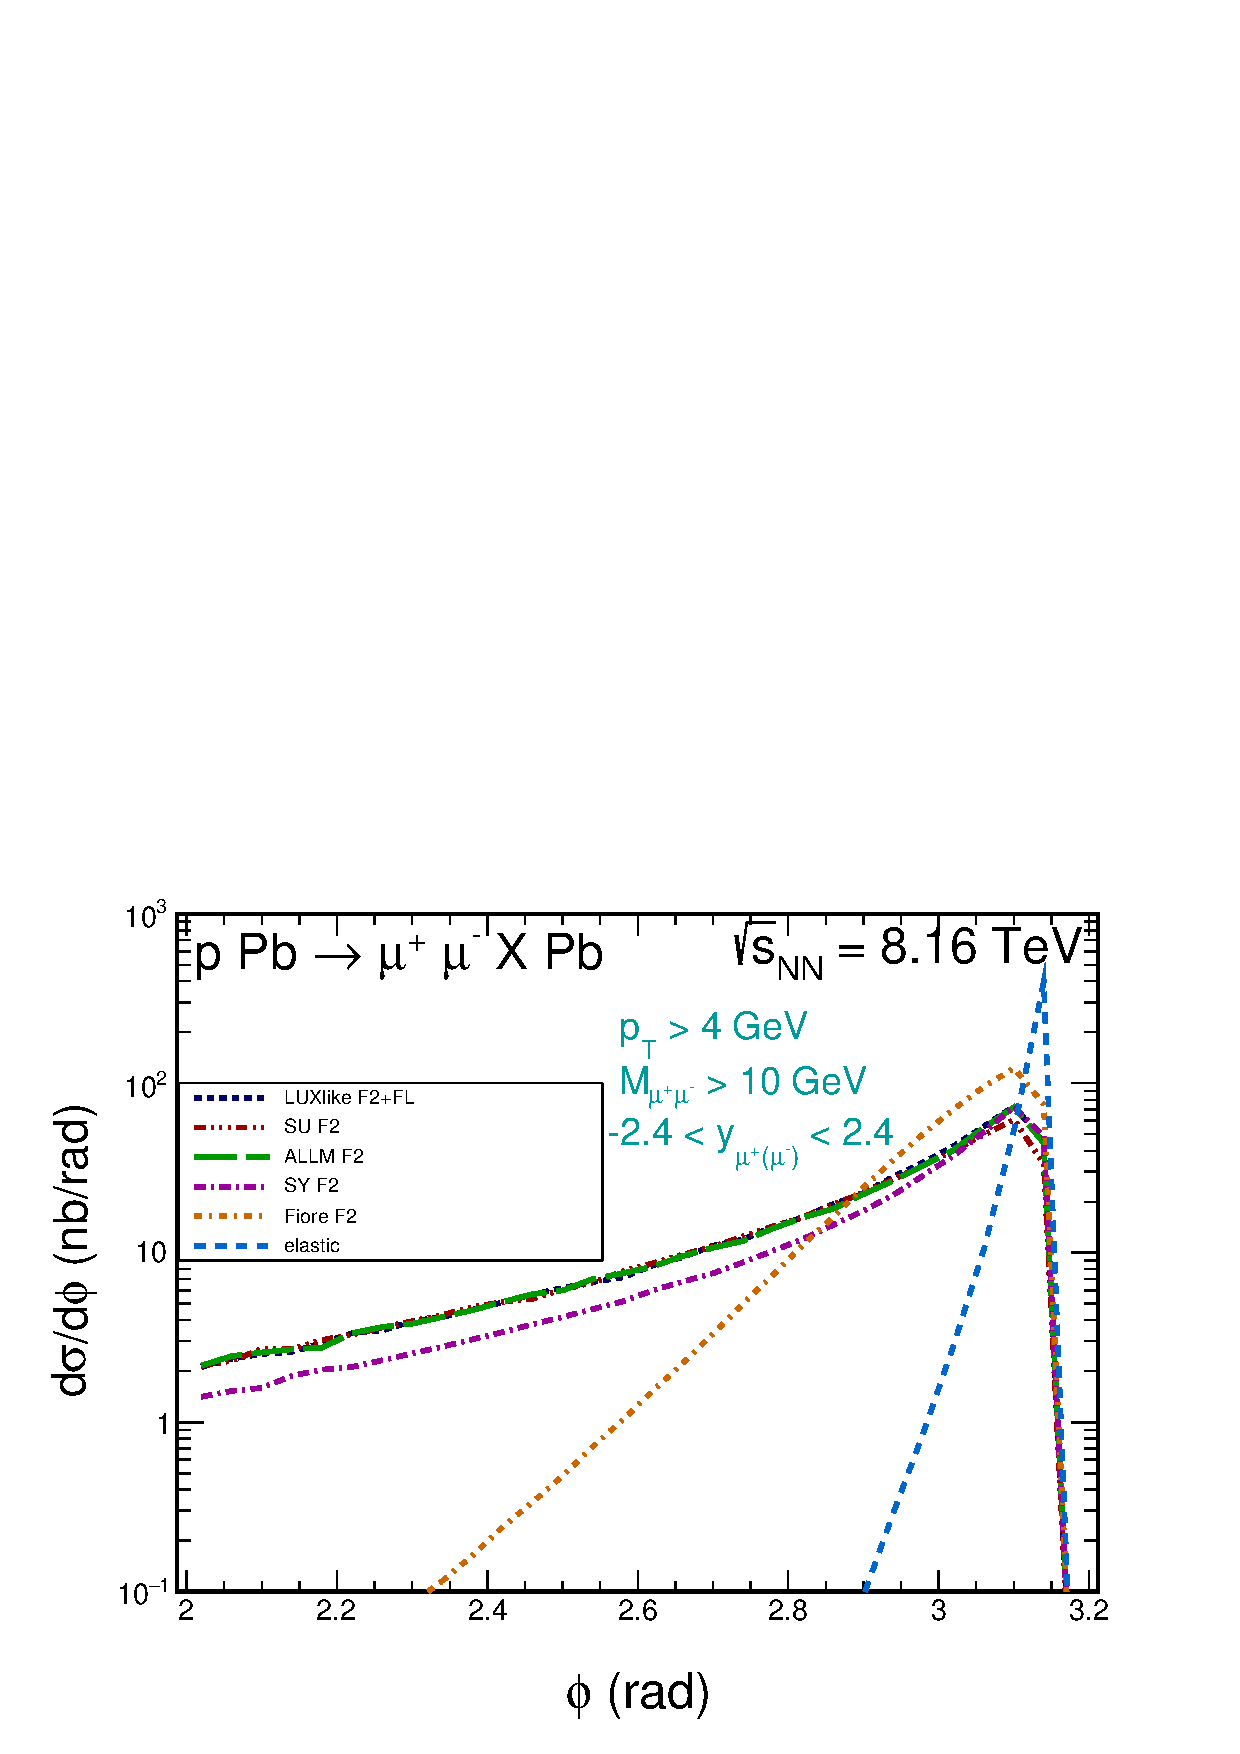
\includegraphics[width=1.0\textwidth]{figures_Marta/phi-c.pdf}}
\end{minipage}
\caption{
Distributions for azimuthal angle between $\mu^+\mu^-$ leptons. (in the left panel we show the results for the whole phase space, while in the right panel only for the fiducial region).
}
\label{fig:dsig_dy}
\end{figure}
%---------------------------------------------------------------





\clearpage
%%%%%%%%%%%%%%%%%%%%%%%%%%%%%%%%%%
\section{Discussion}
\label{sec:discussion}
%%%%%%%%%%%%%%%%%%%%%%%%%%%%%%%%%%

Figure~\ref{fig:inc_cut_kt} compares several differential distribution computed using the two approaches. For the collinear approach pure inelastic contribution is estimated by
subtracting elastic part computed following Eq.~\ref{eq:elasticRenat}.
For the invariant mass distribution and lepton pseudorapidity the shapes are similar and
the main difference between the two predictions is observed in the normalization.
For the distribution of the lepton pair rapidity the two predictions agree at larger rapidities while disagreement concentrates
in the central region. The biggest difference is observed for the transverse momentum distribution of the lepton where at low $p_T$ collinear approximation exceeds the estimate
from $k_T$-factorization approach while at high $p_T$ the ordering is reversed.  
This suggests that at low $p_T$ (close to the boundary of the fiducial region) the difference is due to the smearing of dilepton transverse momentum introduced by the $k_T$-factorization approach.

We also take the opportunity to calculate expected number of events for realistic assumption on total integrated luminosity.
Based on the previous $p+\textrm{Pb}$ runs at the LHC, we assume  $\int Ldt= 200~\textrm{nb}^{-1}$.
We also assume possible experimental efficiencies, mainly due to trigger and reconstruction of leptons, which we embed in a single correction factor $C=0.7$.

Table~\ref{fig:numbers} shows the expected number of events for $p+\textrm{Pb}\rightarrow \textrm{Pb} + \ell^+\ell^- + X$ production at $\sqrt{s_{N N}} = 8.16$~\TeV\ and configuration described above. 
Approximately 2500 elastic dilepton events are expected. 
Depending on the calculations, 3400 (collinear with LUXqed17 PDF) or 2400 ($k_T$-factorization with LUX-like $F_2+F_L$) reconstructed inelastic events are predicted. The difference between collinear and $k_T$-factorization can be therefore constrained with large significance, using existing datasets collected by ATLAS and CMS.



\begin{figure}[]
\includegraphics[width=0.43\textwidth]{figures/Mll_inc_cut_kt.pdf}
\includegraphics[width=0.43\textwidth]{figures/RatioMll_inc_cut_kt.pdf}
\includegraphics[width=0.43\textwidth]{figures/Yll_inc_cut_kt.pdf}
\includegraphics[width=0.43\textwidth]{figures/RatioYll_inc_cut_kt.pdf}
\includegraphics[width=0.43\textwidth]{figures/pTl_inc_cut_kt.pdf}
\includegraphics[width=0.43\textwidth]{figures/RatiopTl_inc_cut_kt.pdf}
\includegraphics[width=0.43\textwidth]{figures/etal_inc_cut_kt.pdf}
\includegraphics[width=0.43\textwidth]{figures/Ratioetal_inc_cut_kt.pdf}
\caption{Differential cross sections in the fiducial region for $p+\textrm{Pb}\rightarrow \textrm{Pb} + \ell^+\ell^- + X$ production at $\sqrt{s_{N N}} = 8.16$~\TeV\ for collinear LUXqed17 photon PDF and
for LUX-like $F_2+F_L$ photon PDF with $k_T$-factorization.
Four differential distributions are shown (from top to bottom): invariant mass of lepton pair, pair rapidity, transverse momentum of negatively-charged lepton and its pseudorapidity. Figures on the right show the ratios to LUXqed17 PDF.}
\label{fig:inc_cut_kt}
\end{figure}


\begin{table}[t]
\begin{center}
\begin{tabular}{|l|c|c|}
\hline
Contribution & Expected events ($C=1$) & Expected events ($C=0.7$) \\
\hline
%$\gamma^{p}_{\rm{el}}$ [$b_{min}=0.7fm$] & 45.5(2) nb & 17.3(1) nb\\
%\hline
$\gamma^{p}_{\rm{el}}$  & 3600 & 2500\\ % [Electric]
\hline
$\gamma^{p}_{\rm{inel}}$ [LUXqed17 collinear] & 5600 & 3900 \\
\hline
$\gamma^{p}_{\rm{inel}}$ [LUX-like $F_2+F_L$] & 3400 & 2400 \\
\hline
\end{tabular}
\end{center}
\caption{Expected number of events for $p+\textrm{Pb}\rightarrow \textrm{Pb} + \ell^+\ell^- + X$ production at $\sqrt{s_{N N}} = 8.16$~\TeV\ assuming $\int Ldt= 200~\textrm{nb}^{-1}$. 
Shown are several contributions: purely elastic, inelastic with collinear LUXqed17 PDF and inelastic with $k_T$-factorization and LUX-like $F_2+F_L$ proton structure function parameterization.
An effect of possible experimental efficiencies is shown in last column.}
\label{fig:numbers}
\end{table}


%%%%%%%%%%%%%%%%%%%%%%%%%%%%%%%%%%
\section{Summary}
%%%%%%%%%%%%%%%%%%%%%%%%%%%%%%%%%%

In summary, we propose a method that would unambiguously allow to test and constrain the photon parton distribution at LHC energies.

%%%%%%%%%%%%%%%%%%%%%%%%%%%%%%%%%%



\section*{References}
%\clearpage
\bibliographystyle{elsarticle-harv}
\bibliography{main}


\end{document}

